\par As described above, diKTat is very configurable and user-friendly. But these are not all of its advantages and features. Below will be presented and described unusual and important killer-feature diKTat.

\subsection{Configuration file}
\par
It's worth starting with the configuration files. This is a file in which the user can manually turn rules on and off or configure the rules settings. Below is one of the rules in the configuration file.
\begin{center}
- name: FILE\underline{ }IS\underline{ }TOO\underline{ }LONG\\
	enabled: true\\
	configuration:\\
	maxSize: '2000'\\
	ignoreFolders: ' '\\
\end{center}
Each rule in this file consists of 3 parts: name - the name of the rule, enabled - the ability to enable or disable the rule, configuration - parameters for the rules. With the first two, everything is obvious. The third parameter is less obvious. The configuration is passed "properties" to check in this rule. For example, if you have a rule "FILE\underline{ }IS\underline{ }TOO\underline{ }LONG" - checking the number of lines in a Kotlin file, then the user can configure the maximum number of lines in the file - by changing the "maxSize" in the configuration,or the user can specify paths to folders that do not need to be checked - by writing the path before these daddy in "ignoreFolders". \\

\subsection{Create ASTNode}
\par
Another fuature is a method that allows you to construct a syntax tree from text. Here's an example of how it works:

\begin{figure}[H]
  \centering
  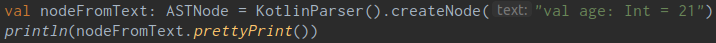
\includegraphics[scale=0.5]{wp/pictures/code.png}
  \caption{Example how to call this method}   
\end{figure}

\begin{figure}[H]
  \centering
  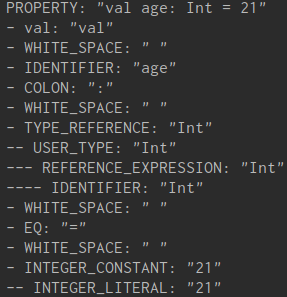
\includegraphics[scale=0.5]{wp/pictures/tree.png}
  \caption{The tree we get}   
\end{figure}

As you can see in the examples, we pass to the method the text of the nodes that we want to receive and the flag, which is set to false by default. The flag should be set to true in order to immediately build a tree with a root node of the FILE type. What's going on inside this method? First of all, the system properties are set (for example: set "idea.io.use.nio2" to true). Further in the method, the text is checked. If the text of the code contains such keywords as import or package, then the method builds a tree with a root node of the FILE type, otherwise it tries with a different root type. In both cases, at the end, if the tree contains an ERROR\underline{ }ELEMENT type of node, it means that an error was made in the code and the method was unable to build the tree and, therefore, throws an exception.\\

\subsection{"SUPPRESS annotation"}
\par
What if the user wants one of the diKTat rules not to check a piece of code? The \textsl{SUPPRESS} annotation will help with this. This annotation can be supplied to ignore a certain rule. For instance, if run this code:

\begin{figure}[H]
  \centering
  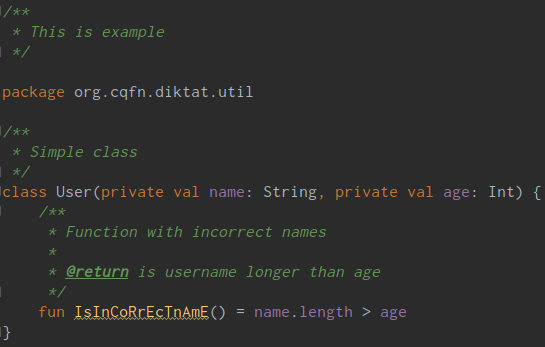
\includegraphics[scale=0.5]{wp/pictures/user_code.png}
  \caption{Example code with incorrect function name}   
\end{figure} 

There will be warning: 

\begin{figure}[H]
  \centering
  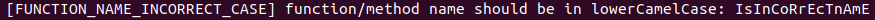
\includegraphics[scale=0.5]{wp/pictures/error.png}
  \caption{Example of warning}   
\end{figure} 

But if there is a \textsl{@SUPPRESS} before this method, then there will be no errors at startup.
\begin{figure}[H]
  \centering
  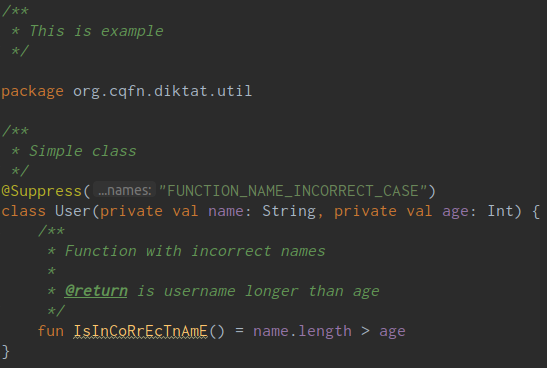
\includegraphics[scale=0.5]{wp/pictures/user_code_with_suppress.png}
  \caption{Example of using "SUPPRESS" annotation}   
\end{figure} 

The example shows that the method has SUPPRESS annotation. Therefore, the \\ FUNCTION\underline{ }NAME\underline{ }INCORRECT\underline{ }CASE rule will be ignored on this method and there will be no error.\\

\subsection{WEB}
\par
Also worth mentioning is the existence of a web version of diKTat.. This is a very handy tool that can be used quickly, and most importantly, it is very simple. A link to it will be below.
\begin{figure}[H]
  \centering
  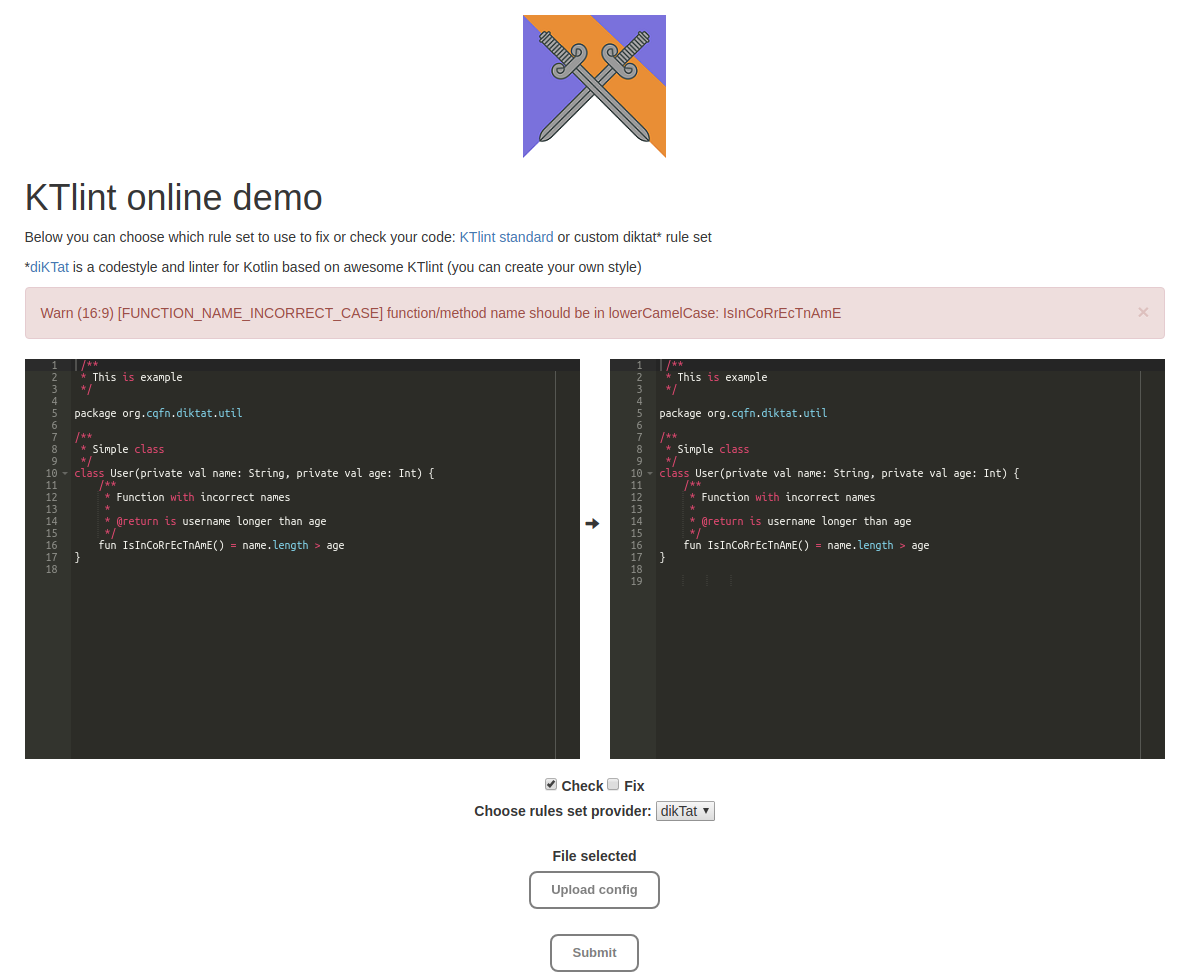
\includegraphics[scale=0.3]{wp/pictures/web-example.png}
  \caption{Example of web application}   
\end{figure} 

\subsection{Validation rules}
\par
As it has been mention earlier, user can customize configuration file on his own but, of course, name of the rule assigned can be incorrect. In this case, diKTat will suggest the closest name based on \textsl{Levenshtein} method.

\subsection{CI-CD}
\par
One of the most important parts of open source project is CI/CD pipeline as it brings considerable benefits to the entire software development process. It improves code quality, customer satisfaction and reduces costs, including time, of making new features.\footnote{The latest version of diKTat you can find here \url{https://github.com/cqfn/diKTat/releases}}.